\documentclass[conference]{IEEEtran}
\IEEEoverridecommandlockouts
\usepackage{cite}
\usepackage{amsmath,amssymb,amsfonts}
\usepackage{graphicx}
\usepackage{textcomp}
% Tectonic/XeTeX uses TU encoding, where IEEEtran's requested Times (ptm) and
% Courier (pcr) shapes are undefined -- bold silently degrades to medium.
% newtx supplies Times-compatible text and math with correct bold shapes.
\usepackage{newtxtext,newtxmath}
\usepackage{xcolor}
\usepackage{booktabs}
\usepackage{array}
\graphicspath{{figures/}}

\begin{document}

\title{Two-Stream Spatial--Temporal Fusion for River\\
Water Quality Prediction with Anomaly\\
Screening and Source Shortlisting}

\author{
\IEEEauthorblockN{Nithyasree Ganesan, Raghav Subramaniam, Tejas Karthikeyan}
\IEEEauthorblockA{Department of Information Science and Technology\\
College of Engineering Guindy, Anna University\\
Chennai -- 600025, India}
}

\maketitle

\begin{abstract}
A purely autoregressive water quality model can learn when parameters move but
not how far, because amplitude is set by catchment conditions absent from a
station's own history. This paper presents a two-stream architecture that
supplies the missing information. A temporal expert applies CEEMDAN
decomposition followed by a CNN--BiLSTM with self-attention; a spatial expert
derives 200 features from Sentinel-2 and Landsat-8 imagery over each station's
catchment, selects a compact subset by evolutionary search, and regresses them
with a random forest. An attention gate learns per-sample weights over the two
experts. Evaluated on 4{,}048 daily records from seven Danube stations
(2012--2023), fusion raises $R^2$ to 0.612 for nitrate-N, 0.459 for dissolved
oxygen and 0.410 for electrical conductance, against 0.517, 0.322 and 0.312 for
the temporal stream alone. We further compare four hyperparameter and feature
selection strategies, finding CMA-ES feature selection improves mean fused
$R^2$ by 21\% over a genetic algorithm while reducing tuning time by 15\%. A
downstream layer screens anomalies by dual rolling-median and seasonal tests,
bounds the search region to a river stretch by cross-station comparison, and
shortlists candidate industrial sites for investigation.
\end{abstract}

\begin{IEEEkeywords}
Water quality prediction, sensor fusion, CEEMDAN, BiLSTM, random forest,
CMA-ES, remote sensing, anomaly screening
\end{IEEEkeywords}

\section{Introduction}

Predicting river water quality is difficult because measurements are nonlinear,
nonstationary, noisy and sparsely sampled. Phase~1 of this project addressed
the temporal side of that problem with a CEEMDAN--CNN--LSTM model incorporating
self-attention, and produced a diagnostic result that determined the direction
of the present work. That model tracked seasonally driven parameters in correct
phase but reproduced only 65--73\% of their observed variance, and recovered no
structure at all for parameters governed by episodic external forcing. In
short, it learned \emph{when} parameters move but not \emph{how far}.

The interpretation is that the missing information is not temporal but spatial.
Amplitude and event timing in a river are governed largely by catchment
conditions -- rainfall and runoff, land use, upstream discharge, sediment
transport -- none of which appear in a station's own measurement history.
Remote sensing supplies exactly this class of
observation~\cite{gholizadeh,sagan,pahlevan}, and is complementary to what a
sequence model already provides.

Phase~2 therefore builds a \emph{spatial expert} over remotely sensed
catchment features and fuses it with the temporal expert under a learned gate,
following the mixture-of-experts principle~\cite{jacobs} in which a gating
network arbitrates between specialists per input. The system was rebuilt on the
Danube, whose record is denser than the sparse gauge data of Phase~1 and whose
seven Serbian stations lie along a single channel, permitting spatial
reasoning. Our contributions are: a two-stream fusion architecture with an interpretable
attention gate; a controlled comparison of four hyperparameter and
feature-selection strategies; and an anomaly screening layer that bounds events
to a river stretch and shortlists candidate industrial sites.

\section{Related Work}

Zhu et al.~\cite{zhu} decompose raw series with CEEMDAN before an LSTM--CNN
network with self-attention, reporting strong accuracy for dissolved oxygen and
pH; this motivated the temporal stream. Yan and Wang~\cite{yan} model Yellow
River Basin stations as graph nodes, combining graph convolution with
reinforcement learning to capture spatial dependency between sites, and
demonstrate that inter-station structure carries predictive signal that
single-site models discard.

For the spatial side, reviews of remote sensing for water quality
retrieval~\cite{gholizadeh,sagan} establish that catchment-scale spectral
information carries signal about nutrient and sediment loading, and Pahlevan et
al.~\cite{pahlevan} demonstrate operational chlorophyll-a retrieval from
Sentinel-2 and Sentinel-3. Shu et al.~\cite{shu} combine super-resolved imagery
with field measurements for groundwater mapping, weighting parameters by fuzzy
AHP. These establish satellite imagery as a viable predictor source but
typically use it in isolation rather than fused with a temporal model.

On optimisation, random search is a strong hyperparameter
baseline~\cite{bergstra}; Optuna's TPE~\cite{akiba} models the objective
density and BOHB~\cite{falkner} adds successive halving for efficiency. For
feature selection, genetic algorithms~\cite{holland,dash} are conventional,
while CMA-ES~\cite{hansen} adapts a full covariance model of the search
distribution, suiting correlated landscapes -- a plausible description of a
spectral feature space with strongly intercorrelated bands and indices. We test
that in Section~V. Across this literature, results are often reported without
baselines or per-component ablations, making it hard to establish where
accuracy originates; we report per-stream metrics throughout.

\section{System Architecture}

The system comprises four layers: acquisition and preprocessing, the two-stream
predictor, the fusion gate, and anomaly screening.

\subsection{Temporal Expert Stream}

Twelve signals per station -- streamflow, precipitation, water temperature and
nine spectral bands -- are decomposed by CEEMDAN~\cite{torres} into intrinsic
mode functions, isolating oscillatory modes from high-frequency noise to
low-frequency trend:

\begin{equation}
X(t) = \sum_{k=1}^{N} \mathrm{IMF}_k(t) + r_N(t)
\end{equation}

The resulting 134-channel representation over a 30-day window passes through a
1-D CNN for local feature extraction, a bidirectional LSTM~\cite{hochreiter}
for longer-range dependency, and a self-attention layer~\cite{vaswani} that
performs learned weighted pooling over the sequence, so each historical step's
contribution is explicitly weighted.

\subsection{Spatial Expert Stream}

For each station and date, nine spectral bands (Blue through SWIR2, including
three red-edge bands) and sixteen derived indices are computed. Beyond standard
indices such as NDWI, NDVI and NDTI, several are domain-specific: a clay index
and particle-size proxy marking phosphorus-adsorbing soil runoff, a dilution
proxy relating conductance to discharge, and a Garcia--Gordon dissolved oxygen
saturation term giving the physical upper bound at measured temperature. Each
of the 25 base features is summarised over a 30-day window by seven statistics,
giving 200 spatial features.

This dimensionality far exceeds the available measurements, so a compact subset
is selected by evolutionary search -- either a genetic
algorithm~\cite{holland} with $L_0$ penalty on the number of selected
features, or CMA-ES~\cite{hansen} over a continuous relaxation -- and regressed
with a random forest~\cite{breiman}, which is well suited to the resulting
small-sample, high-dimensional regime.

\subsection{Attention Fusion Gate}

Rather than averaging the two experts, a gating network computes per-sample
weights from the concatenated temporal hidden state $\mathbf{h}_t$, spatial
feature vector $\mathbf{f}_s$ and an encoded hydro-meteorological context
$\mathbf{c}$:

\begin{equation}
[w_t, w_s] = \mathrm{softmax}\big(\mathbf{W}_2\,\mathrm{ReLU}(\mathbf{W}_1[\mathbf{h}_t;\mathbf{f}_s;\mathbf{c}])\big)
\end{equation}
\begin{equation}
\hat{y} = w_t\,\hat{y}_{\text{temporal}} + w_s\,\hat{y}_{\text{spatial}}
\end{equation}

Because $w_t + w_s = 1$ and both are produced per sample, the gate is directly
interpretable: it reports which expert the model relied on for each prediction.

\subsection{Anomaly Screening and Source Shortlisting}

This layer is decision support: it narrows where an investigator should look
and does not determine causation, for reasons Section~V-C sets out.

Anomalies are screened on measured values rather than predictions, using two
tests that must both fire: a rolling Z-score against a 90-day median and MAD,
and a seasonal test against the same-month mean across all years. Requiring
both suppresses false positives from seasonal extremes, and events are
classified \emph{acute} or \emph{trend} by whether the rolling mean is itself
elevated. Because the seven stations lie along one channel at known river
kilometres, the most upstream station showing an anomaly bounds the search
region to the stretch above it -- a geometric constraint, independent of any
assumption about cause.

Industrial facilities within that stretch are retrieved from an OpenStreetMap
database via the Overpass API and filtered by pollutant compatibility, giving a
shortlist of sites whose effluent profile could in principle produce the
observed signature. Events exceeding $Z \geq 3.5$ are routed to a large
language model, which receives the measurement, baselines, multi-station
context and shortlist, and returns ranked hypotheses with stated confidence and
follow-up checks. Proximity and pollutant compatibility justify inclusion in a
shortlist, not a finding of discharge; outputs are investigative leads
requiring field verification.

\section{Implementation}

\subsection{Dataset}

The Danube dataset covers seven Serbian monitoring stations from Bezdan
(km~1425) to Tekija, spanning 1~December~2012 to 31~December~2023 -- 4{,}048
daily records per station. Water quality targets are dissolved oxygen, total
phosphorus, nitrate-N, electrical conductance and chlorophyll-a, drawn from
GFQA records at 125--180 samples per station per parameter. Satellite
observations come from Sentinel-2 and Landsat-8; discharge, precipitation and
water temperature provide hydro-meteorological context.

Two preprocessing issues required correction. Google Earth Engine exported
dates in day-of-year form (e.g.\ \texttt{2013-04-118}), which parses silently
but wrongly unless the third field is detected as a DOY when it exceeds 31.
Landsat-8 lacks red-edge bands and encodes them as $-9999$; these were
converted to missing and interpolated from Sentinel-2 rather than treated as
valid reflectance.

Critically, water quality targets are used only on actual measurement dates.
Interpolating targets to a daily grid inflates apparent performance
catastrophically, since the model then learns the interpolator rather than the
process; input features may be interpolated, but labels may not.

\subsection{Training and Optimisation}

Models are implemented in PyTorch with Metal Performance Shaders acceleration.
Training uses a masked MSE loss so that missing targets contribute no gradient,
with early stopping on validation loss. Splits are chronological, never random.

Four tuning strategies were compared under identical architecture and data,
varying only how hyperparameters are chosen and how spatial features are
selected: random search with GA selection (the baseline), Optuna
TPE~\cite{akiba} with GA, BOHB~\cite{falkner} with GA, and random search with
CMA-ES selection. Each used 3-fold cross-validation; results are reported on
135 held-out test samples.

\section{Results}

\subsection{Stream Contributions}

Table~\ref{tab:streams} reports $R^2$ for each stream under the best
configuration, and Fig.~\ref{fig:streams} shows the same comparison.

\begin{table}[!t]
\caption{Per-Stream $R^2$, Random Search + CMA-ES (135 Test Samples)}
\label{tab:streams}
\centering
\small
\setlength{\tabcolsep}{4pt}
\begin{tabular}{lrrr}
\toprule
\textbf{Parameter} & \textbf{Temporal} & \textbf{Spatial} & \textbf{Fused} \\
\midrule
Dissolved oxygen        & 0.322 & \textbf{0.629} & 0.459 \\
Nitrate-N               & 0.517 & 0.384 & \textbf{0.612} \\
Electrical conductance  & 0.312 & 0.395 & \textbf{0.410} \\
Chlorophyll-a           & 0.129 & $-0.255$ & \textbf{0.285} \\
Total phosphorus        & $-0.121$ & 0.004 & $-0.052$ \\
\bottomrule
\end{tabular}
\end{table}

\begin{figure}[!t]
\centering
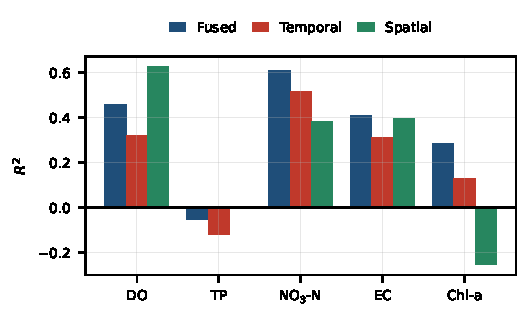
\includegraphics[width=\columnwidth]{fig_streams.pdf}
\caption{Per-stream $R^2$ across the five targets. Fusion exceeds both
individual experts for nitrate-N, conductance and chlorophyll-a, but not for
dissolved oxygen, where the spatial stream alone is stronger.}
\label{fig:streams}
\end{figure}

Fusion improves on the temporal stream for every parameter, confirming the
Phase~1 hypothesis that spatial information supplies signal a sequence model
cannot recover alone. Gains are substantial: nitrate-N rises from 0.517 to
0.612, conductance from 0.312 to 0.410, and chlorophyll-a from 0.129 to 0.285.

Two results deserve emphasis because they complicate the simple reading. For
dissolved oxygen the spatial stream alone attains $R^2 = 0.629$, well above the
fused 0.459 -- the gate dilutes a strong expert with a weaker one. For
chlorophyll-a the opposite holds: fusion (0.285) beats both temporal (0.129)
and spatial ($-0.255$) streams, so the gate extracts value from an expert that
is worse than useless on its own. Total phosphorus remains negative across all
configurations, which is consistent with its measurement scale: values below
0.05~mg/L sit near the analytical detection limit, so a large fraction of the
observed variance is measurement noise rather than signal.

The mean attention weights are 0.817 temporal and 0.184 spatial. The gate
therefore leans heavily on the temporal expert overall, despite the spatial
expert being the stronger predictor for dissolved oxygen and conductance. This
imbalance, combined with the dissolved oxygen result, indicates the gate is
under-trained relative to the streams it arbitrates and is the most promising
target for further work.

\subsection{Optimisation Strategy Comparison}

Table~\ref{tab:hpo} and Fig.~\ref{fig:hpo} compare the four strategies.

\begin{table}[!t]
\caption{Tuning Strategy Comparison (3-Fold CV, 135 Test Samples)}
\label{tab:hpo}
\centering
\small
\setlength{\tabcolsep}{3pt}
\begin{tabular}{llrrr}
\toprule
\textbf{HPO} & \textbf{Feat.\ sel.} & \textbf{Trials} & \textbf{Time (min)} & \textbf{Mean $R^2$} \\
\midrule
Random & GA      & 12 & 214 & 0.326 \\
TPE    & GA      & 20 & 318 & 0.365 \\
BOHB   & GA      & 22 & 197 & 0.360 \\
Random & CMA-ES  & 12 & \textbf{183} & \textbf{0.442} \\
\bottomrule
\end{tabular}
\end{table}

\begin{figure}[!t]
\centering
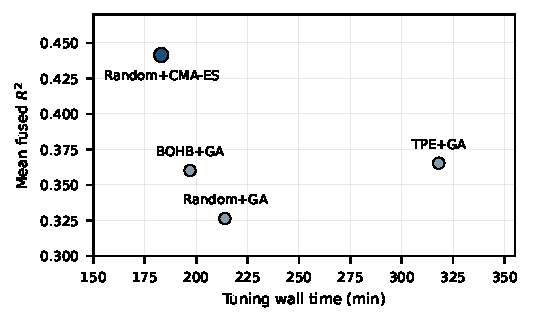
\includegraphics[width=\columnwidth]{fig_hpo.pdf}
\caption{Mean fused $R^2$ against tuning wall time. CMA-ES feature selection
dominates: highest accuracy at the lowest cost.}
\label{fig:hpo}
\end{figure}

The comparison isolates a clear effect. Changing the \emph{hyperparameter}
search from random to TPE or BOHB yields modest gains (0.326 to 0.365 and
0.360), at 49\% more wall time for TPE. Changing the \emph{feature selector}
from GA to CMA-ES, while holding random search fixed, lifts mean fused $R^2$
to 0.442 -- a 21\% improvement over the best GA variant -- while reducing
tuning time to 183 minutes, the fastest of the four. Per-parameter gains over
the GA baseline are $+7.1\%$ for dissolved oxygen, $+10.3\%$ for nitrate-N,
$+11.2\%$ for conductance and $+17.6\%$ for chlorophyll-a. CMA-ES converged in
12.4 generations on average against 20 for the GA.

The magnitude of this result relative to the hyperparameter effect suggests
that on this problem, \emph{which spectral features enter the spatial expert}
matters considerably more than how the network is configured. This is
consistent with the intercorrelated structure of a spectral feature space, in
which CMA-ES's covariance model is better matched to the search landscape than
the GA's independent bit-flips. We note the comparison rests on a single seed
per configuration, so the ranking of TPE against BOHB is within plausible
run-to-run variance; the CMA-ES margin is large enough to be robust to it.

\subsection{Anomaly Screening: Scope and Evaluation Limits}

On the historical record the screen flags events passing both the rolling and
seasonal tests. A representative case is an electrical conductance reading of
387~$\mu$S/cm at Bogojevo on 10~October~2017 against a rolling median of
350~$\mu$S/cm, giving a rolling Z of 16.6 and classification as acute. With
only that station affected, the search region is bounded to the 58~km stretch
between Bezdan (km~1425) and Bogojevo (km~1367). No facility in the industrial
database matched this stretch and pollutant, which the report records
explicitly rather than returning a source.

We report no precision, recall or attribution accuracy here, because the
required ground truth does not exist in our evaluation set. Validation would
need dated incident logs, to separate genuine events from sensor faults and
natural low-flow spikes; reported discharge locations, to test the bounded
stretch; and verified responsible parties, to test the shortlist. For the
Danube the ICPDR Accident Emergency Warning System and the European Pollutant
Release and Transfer Register are candidate sources, though the latter is
annual and constrains plausibility rather than timing.

Absent that evidence, a statistical outlier cannot be distinguished from a
pollution event, nor proximity from responsibility. We therefore position this
layer as triage that reduces an investigator's search space from an eleven-year
multi-station record to a few dated, spatially bounded events -- which the
present evaluation does support -- and claim no ability to identify
polluters.

\section{Conclusion}

This work built a two-stream spatial--temporal architecture in direct response
to a Phase~1 finding: that a temporal model learns when water quality
parameters move but not how far, because amplitude is governed by catchment
conditions absent from station history. Adding a spatial expert over
remotely sensed catchment features and fusing it under a learned attention gate
improved $R^2$ on every parameter relative to the temporal stream alone,
reaching 0.612 for nitrate-N, 0.459 for dissolved oxygen and 0.410 for
conductance. The Phase~1 hypothesis is therefore supported.

The tuning comparison produced the study's most transferable result:
substituting CMA-ES for a genetic algorithm as the spatial feature selector
improved mean fused $R^2$ by 21\% while reducing tuning time by 15\%,
outweighing the hyperparameter search strategy. For intercorrelated spectral
features, feature selection appears the higher-leverage choice.

Two limitations bound these conclusions. The gate assigns 0.817 mean weight to
the temporal stream despite the spatial expert being stronger for dissolved
oxygen, where fusion scores 0.459 against 0.629 -- leaving accuracy unclaimed
and warranting a per-target rather than per-sample formulation. Total
phosphorus stays unpredictable throughout, which we attribute to measurement
noise near the detection limit rather than model capacity: a data problem no
architecture change resolves.

A third limitation is evidential rather than technical: without confirmed
incident records we cannot show that a flagged outlier is a pollution event,
nor that a shortlisted facility discharged anything. We therefore scope this
component as investigative triage rather than attribution.

Future work follows from all three. The gate should be trained with the streams
frozen so it learns arbitration rather than co-adapting; per-target gating
would let it defer to the spatial expert where that expert is demonstrably
better. Extending the design so neighbouring stations inform one another,
following the graph-based direction of Yan and Wang~\cite{yan}, would exploit
the same channel geometry the screening layer already uses to bound its search
region. Validating that layer will require linking flagged events to
independent incident records, most plausibly as a small case-study series
given how rarely confirmed events occur.

\begin{thebibliography}{00}

\bibitem{zhu} M. Zhu et al., ``A hybrid CEEMDAN--LSTM--CNN model with
self-attention for water quality prediction,'' \emph{Environmental Modelling
\& Software}, 2023.

\bibitem{yan} X. Yan and Y. Wang, ``GARL: Graph convolution autoencoder
reinforcement learning network for water quality prediction in the Yellow River
Basin,'' \emph{Journal of Hydrology}, 2023.

\bibitem{shu} L. Shu et al., ``Deep learning-based groundwater quality
monitoring using super-resolution satellite imagery and fuzzy AHP,''
\emph{Water Resources Research}, 2023.

\bibitem{torres} M. E. Torres, M. A. Colominas, G. Schlotthauer, and P.
Flandrin, ``A complete ensemble empirical mode decomposition with adaptive
noise,'' in \emph{Proc. IEEE ICASSP}, 2011, pp. 4144--4147.

\bibitem{hochreiter} S. Hochreiter and J. Schmidhuber, ``Long short-term
memory,'' \emph{Neural Computation}, vol. 9, no. 8, pp. 1735--1780, 1997.

\bibitem{vaswani} A. Vaswani et al., ``Attention is all you need,'' in
\emph{Proc. NeurIPS}, 2017, pp. 5998--6008.

\bibitem{breiman} L. Breiman, ``Random forests,'' \emph{Machine Learning},
vol. 45, no. 1, pp. 5--32, 2001.

\bibitem{jacobs} R. A. Jacobs, M. I. Jordan, S. J. Nowlan, and G. E. Hinton,
``Adaptive mixtures of local experts,'' \emph{Neural Computation}, vol. 3,
no. 1, pp. 79--87, 1991.

\bibitem{holland} J. H. Holland, \emph{Adaptation in Natural and Artificial
Systems}. Ann Arbor, MI: University of Michigan Press, 1975.

\bibitem{dash} M. Dash and H. Liu, ``Feature selection for classification,''
\emph{Intelligent Data Analysis}, vol. 1, no. 3, pp. 131--156, 1997.

\bibitem{hansen} N. Hansen and A. Ostermeier, ``Completely derandomized
self-adaptation in evolution strategies,'' \emph{Evolutionary Computation},
vol. 9, no. 2, pp. 159--195, 2001.

\bibitem{bergstra} J. Bergstra and Y. Bengio, ``Random search for
hyper-parameter optimization,'' \emph{Journal of Machine Learning Research},
vol. 13, pp. 281--305, 2012.

\bibitem{akiba} T. Akiba, S. Sano, T. Yanase, T. Ohta, and M. Koyama,
``Optuna: a next-generation hyperparameter optimization framework,'' in
\emph{Proc. ACM SIGKDD}, 2019, pp. 2623--2631.

\bibitem{falkner} S. Falkner, A. Klein, and F. Hutter, ``BOHB: robust and
efficient hyperparameter optimization at scale,'' in \emph{Proc. ICML}, 2018,
pp. 1437--1446.

\bibitem{gholizadeh} M. H. Gholizadeh, A. M. Melesse, and L. Reddi, ``A
comprehensive review on water quality parameters estimation using remote
sensing techniques,'' \emph{Sensors}, vol. 16, no. 8, art. 1298, 2016.

\bibitem{sagan} V. Sagan et al., ``Monitoring inland water quality using
remote sensing: potential and limitations of spectral indices, bio-optical
simulations, machine learning, and cloud computing,'' \emph{Earth-Science
Reviews}, vol. 205, art. 103187, 2020.

\bibitem{pahlevan} N. Pahlevan et al., ``Seamless retrievals of chlorophyll-a
from Sentinel-2 (MSI) and Sentinel-3 (OLCI) in inland and coastal waters,''
\emph{Remote Sensing of Environment}, vol. 240, art. 111604, 2020.

\end{thebibliography}

\end{document}
